\documentclass{bioinfo}
\copyrightyear{2018} \pubyear{2018}

\access{Advance Access Publication Date: Day Month Year}
\appnotes{Manuscript Category}

\begin{document}
\firstpage{1}

\subtitle{Biostatistics \& Medical Informatics 776: Advanced Bioinformatics Project}

\title[short Title]{miRNA Normalization and Amplification Bias}
\author[Sample \textit{et~al}.]{John Steill\,$^{\text{\sfb 1,}*}$}
\address{$^{\text{\sf 1}}$Biostatistics \& Medical Informatics, University of Wisconsin, Madison, WI, 53792.}
\corresp{$^\ast$To whom correspondence should be addressed.}

\history{May 11, 2018}

\editor{}

\abstract{\textbf{Motivation:} Small noncoding RNAs known as microRNA (miRNA) play a crucial role in gene expression regulation. Each miRNA can target many genes, and many genes can be affected by a variety of miRNA. However, there is still no consensus on how expression data should be pre-processed before downstream analysis. This work surveys and evaluates existing normalization methods and characterizes amplification biases. By sequencing samples which are biological replicates but different technical preparations, we seek to minimize the false positives in differentially expressed miRNA librariesfrom technical replicates\\
\textbf{Results:} .\\
\textbf{Availability:} https://github.com/JohnWSteill/bmi776\_miRNA\_project.git \\
\textbf{Contact:} \href{jsteill@morgridge.org}{jsteill@morgridge.org}\\
\textbf{Supplementary information:} Supplementary data available upon request.}

\maketitle

\section{Introduction}
The problem of comparing RNA-Seq expression levels among disparate samples has been extensively explored.  \citep{Conesa16} Many successful methods are motivated by first making assumptions about what the researcher roughly expects and working backwards. For example, if the highest expressers are considered housekeeping genes and are not of interest in the experiment, it would make sense to use an upper quartile (or higher) normalization. On the other hand, if the highest expressed genes are expected to vary, the effects of relative abundance will be marked, and it would be appropriate to use a median-by-ratio normalization method. Without any such knowledge, we may choose to use simple TPM for a first exploratory pass. \vspace{4pt} \\ 
miRNA normalization is especially challenging. There are fewer varieties, and we may see many fewer libraries being simultaneously expressed. We also may be comparing samples in which the number expressed vary greatly (as well as expression magnitudes.) Finally, technically we often struggle to get enough biological material and forces to use smaller amounts and more amplification cycles than desired, which introduces another source of bias.  \vspace{4pt} \\
For this study, an ideal normalization is one which produces no differentially expressed libraries, because they are all biological replicates. My hypothesis is we see the fewest false positive DE miRNAs from a very high quantile normalization. This may distort lower-expressed miRNAs, but this will be mitigated because it requires a higher fold change to trigger a differentially expressed threshold with fewer raw counts. If the highest expresser shows significant amplification bias, this hypothesis may be proved incorrect. \\

\begin{methods}
\section{Methods}
\subsection{Sample Acquisition}
The samples were motivated from an experiment studying fetal mouse liver development. This study is challenging because few miRNAs are expressed so early and the levels are changing rapidly, which makes normalization non-trivial. In addition, because embryonic mouse livers are on the order of 10 microns, getting enough tissue is difficult, necessitating more amplification.\citep{Xu10}  However, for cost and convenience, a human hepatocyte-like culture induced from a pluripotent cell line was used. The sample was partitioned into 6 samples of amounts of 3.25 ng, 6 of 6.5 ng, 6 of 12.5, and one of 100ng. The 100ng will be taken as a gold standard. Each batch of six was divided into 3 sets of two replicates, which underwent 15, 20, and 30 cycles of PCR amplification.\vspace{4pt} \\  
The samples were prepped with a custom ligation mediated protocol, pooled and sequenced on an Illumina Hi-Seq 3000.  The samples were demultiplexed with Illumina's bcl2fastq 2.17 software to generate fastq files. 
\subsection{Calculation of Expected Counts}
A custom algorithm was developed for mapping reads to families of miRNAs. A family was defined as a group of miRNA that shares the first 15 bases. This is because the larger investigation is centered around the production/inhibition of Albumin and Alpha-Fetoprotein (AFP). The binding sites are small, on the order of 5-8 bases, and we would like to track these populations together. The hsa-mir library was thus reduced: miRNAs which shared the first 15 bases were combined and given a comma-separated name of their constituents.  Alignment was done by creating a hash table with 15-mers as keys, and counts as values.
Figure~1 \vphantom{\ref{fig:1}} shows the ten most prevalent. \\

\vspace{4pt} 
  
\subsection{Normalization Algorithms}
\subsubsection{CPM}
The simplest normalization, shown in Figure \ref{fig:2}, is counts per million (CPM), in which counts are divided by the total number of reads and multiplied by $10^6$. \\

\subsubsection{Tam Upper Quartile}
As mentioned previously, traditional upper quartile normalization from RNA-Seq studies is hampered by the relatively large number of low expressed libraries. Even if we restrict ourselves to non-zero values, the $75^{\text{th}}$ percentile would give expected counts in the low single digits.  \citep{Tam15} addressed this by a two-step filter: first we limit the set of miRNAs to those with an expected count of 5 or greater, and then take the $75^{\text{th}}$ percentile of the miRNAs remaining. In practice, this is equivalent to using a 95\% percentile normalization. Again for the top expressers, this is shown in Figure \ref{fig:3}.
\subsubsection{TMM}
Finally, we will examine the TMM algorithm, as implemented in edgeR \citep{McCarthy12}  package. This method, introduced by \citep{Robinson10} first estimates a dispersion, and then finds a mean after discarding a fraction of the top and bottom of the data. This normalization is shown in Figure \ref{fig:4}.
\subsection{Finding Bias Candidates with a Generalized Linear Model}
To build a generalized linear model, we use the number of cycles and the starting amounts as design variables. Thus there are three levels to the cycle variable: 15, 20, and 30 cycles. There are four starting amounts: 3ng, 6ng, 13ng, and 100ng. 
our model is therefore: \\
\begin{equation}
M = \text{\textasciitilde}\text{\it{Amt}}+\text{\it{Ncycles}}\label{eq:01}
\end{equation}
The edgeR package also supports a general linear model. I largely followed the tutorial from \citep{Rueda15}.
\end{methods}

\section{Results}
\subsection{Normalization Comparison}
The Tam UQ normalization was superior, as it the fewest false positives, 46, using edgeR's default settings. The TMM and CPM algorithms both gave 77 false positives. (There were approximately 400 miRNAs which were expressed at >1 CPM.) 

\subsection{GLM characterization of amplification bias}
Table \ref{tab:1} gives the coefficients of the linear model for the top expressers. Values are expressed in base log2.


\section{Discussion}

In Figure \ref{fig:1}, we can see that even with the maximum number of 30 pcr cycles, the total number of reads was less than the gold standard case. This is important because as it appears there still was some room to grow, and the concentrations were not saturated. So it's likely that all libraries were being amplified, but at different rates. Although we will see this more clearly subsequently, note the differing trajectories of hsa-let-7f-5p (solid orange) and hsa-miR-151a-3p (dashed green), at the bottom of the page. For all initial starting conditions, the concentrations are on par for 15 cycles, but the former consistently outstrips the latter as the number of cycles increases. \vspace{4pt} \\
This same behavior can be seen more clearly in other miRNAs in Figure \ref{fig:2}. hsa-miR-26a-5p, hsa-miR-30d-5p, and the hsa-miR-146* family all consistently gain a greater share of the total reads as the number of cycles increase. To investigate what  these varieties have in common, I first examined their relative CG content, and then the folding prediction from Mfold webserver \citep{Zuker03}. Neither showed an obvious correlation.  For this aim I was unable to find an expanation as to why some libraries show consistent relative increase with cycles. Future work could involve inspecting more miRNAs, as well as modfying Mfold's default parameters. It may be that even though the most stable configuration is linear, some folding is constantly occuring and breaking, affecting the kinetics of amplification. \vspace{4pt} \\
Even the "flat" species are interesting, because although like the gold standard they are the most highly expressed, they are a very different proportion. There is a possibility of batch effects, as the gold standard sample was run on a different flowcell. A final insight from Figure \ref{fig:2} is that there is no single normalization strategy that will not have one of the top two libraries being viewed as differentially expressed; there is a fold change of about 3 that must be divided among the two.  \vspace{4pt} \\
Figure \ref{fig:3} appears to attempt to do this, with both miRNAs falling. Recall the normalization constant was the $75^{\text{th}}$ percentile of the miRNAs with a count above 5, or about rank 125. Even though this is still far away from the top 10, qualitatively we see much of the signal which was responding to the cycle number has been muted. This qualitative observation matches the conclusion from edgeR, which minimized false positives with this normalization. \vspace{4pt} \\
The values in Table \ref{tab:1} correspond to this normalization. Much of this table is merely restating what we've already observed visually, the larger coefficients for C20 and C30 correspond to miRNAs we've already examined as up-regulated in Table \ref{tab:2}. \vspace{4pt} \\
Figure \ref{fig:4} looks very similar to Figure \ref{fig:1}, the raw counts. Upon reflection, this must be because the normalization is very close to one. Just as \citep{Tam15} needed to tweak the traditional UQ normalization to account for the many unexpressed libraries, it is evident that a similar step needs to be taken to put TMM on even footing, and edgeR's default algorithm should be re-implemented. 

In conclusion, an upper percentile normalization is the optimal choice, although the optimal percentile is an open question.
Because I didn't have samples which should show differentially expressed miRNA, I avoided attempting to find this. Future work should attempt to balance this with some samples which are known to have some DE miRNA. 

\begin{thebibliography}{}

\bibitem[Conesa {\it et~al}, 2016]{Conesa16}
Conesa, A., Madrigal, P., Tarazona, S., Gomez-Cabrero, D., Cervera, A., McPherson, A., ... \& Mortazavi, A. (2016). A survey of best practices for RNA-seq data analysis. Genome biology, 17(1), 13.

\bibitem[Xu {\it et~al}, 2010]{Xu10}Xu, H., He, J. H., Xiao, Z. D., Zhang, Q. Q., Chen, Y. Q., Zhou, H., \& Qu, L. H. (2010). Liver-enriched transcription factors regulate microRNA-122 that targets CUTL1 during liver development. Hepatology, 52(4), 1431-1442.

\bibitem[Tam {\it et~al}, 2015]{Tam15} Tam, S., Tsao, M. S., \& McPherson, J. D. (2015). Optimization of miRNA-seq data preprocessing. Briefings in bioinformatics, 16(6), 950-963.

\bibitem[Robinson {\it et~al}, 2010]{Robinson10}Robinson, M. D., \& Oshlack, A. (2010). A scaling normalization method for differential expression analysis of RNA-seq data. Genome biology, 11(3), R25.

\bibitem[McCarthy {\it et~al}, 2012]{McCarthy12}McCarthy DJ, Chen Y \& Smyth GK (2012). Differential expression analysis of multifactor RNA-Seq experiments with respect to biological variation. Nucleic Acids Research 40, 4288-4297

\bibitem[Rueda  {\it et~al}, 2015]{Rueda15}Oscar Rueda \& Bernard Pereira (2015, July 15). Differential Expression Analysis using edgeR. Retrieved from https://bioinformatics-core-shared-training.github.io/cruk-bioinf-sschool/Day3/rnaSeq\_DE.pdf

\bibitem[Zuker  {\it et~al}, 2003]{Zuker03}Zuker, M. (2003). Mfold web server for nucleic acid folding and hybridization prediction. Nucleic acids research, 31(13), 3406-3415.


\end{thebibliography}


\section{Figures and Tables}
\onecolumn


\begin{figure}[!tpb]
\centerline{\includegraphics[scale=0.7]{fig-1-raw.eps}}
\caption{Expected Counts of miRNA groups}\label{fig:1}
\end{figure}

\begin{figure}[!tpb]
\centerline{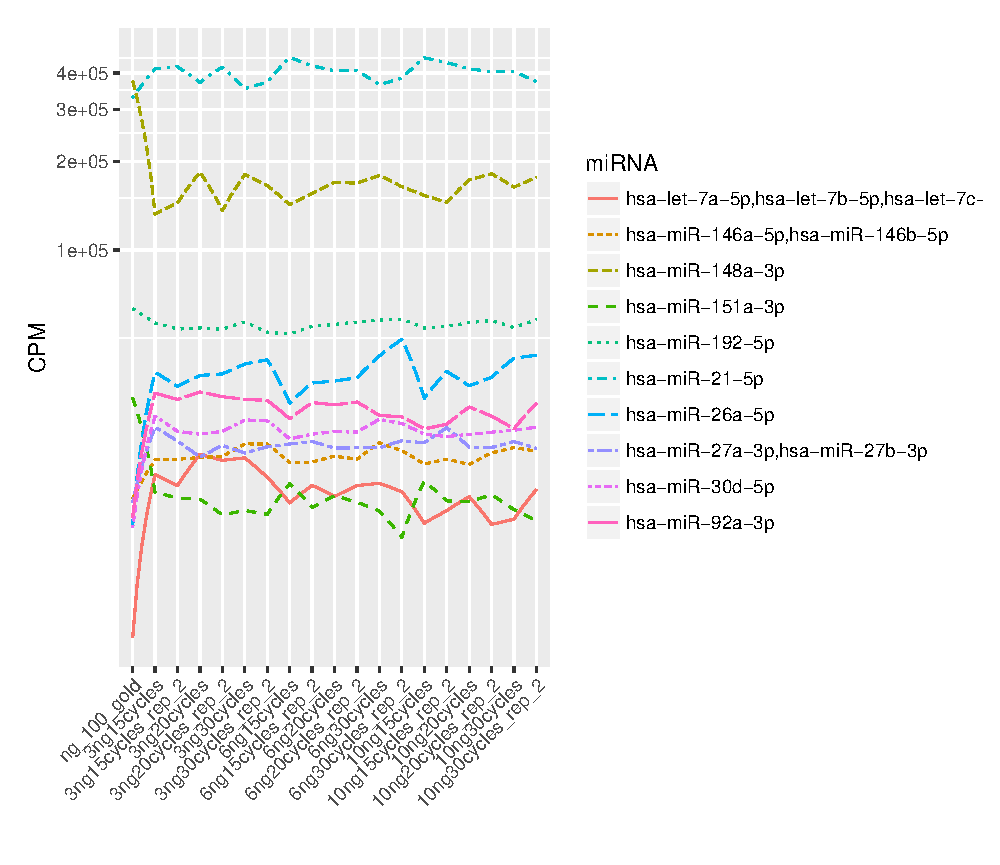
\includegraphics[scale=0.7]{Fig-2-cpm.eps}}
\caption{CPM Normalization}\label{fig:2}
\end{figure} 


\begin{figure}[!tpb]
\centerline{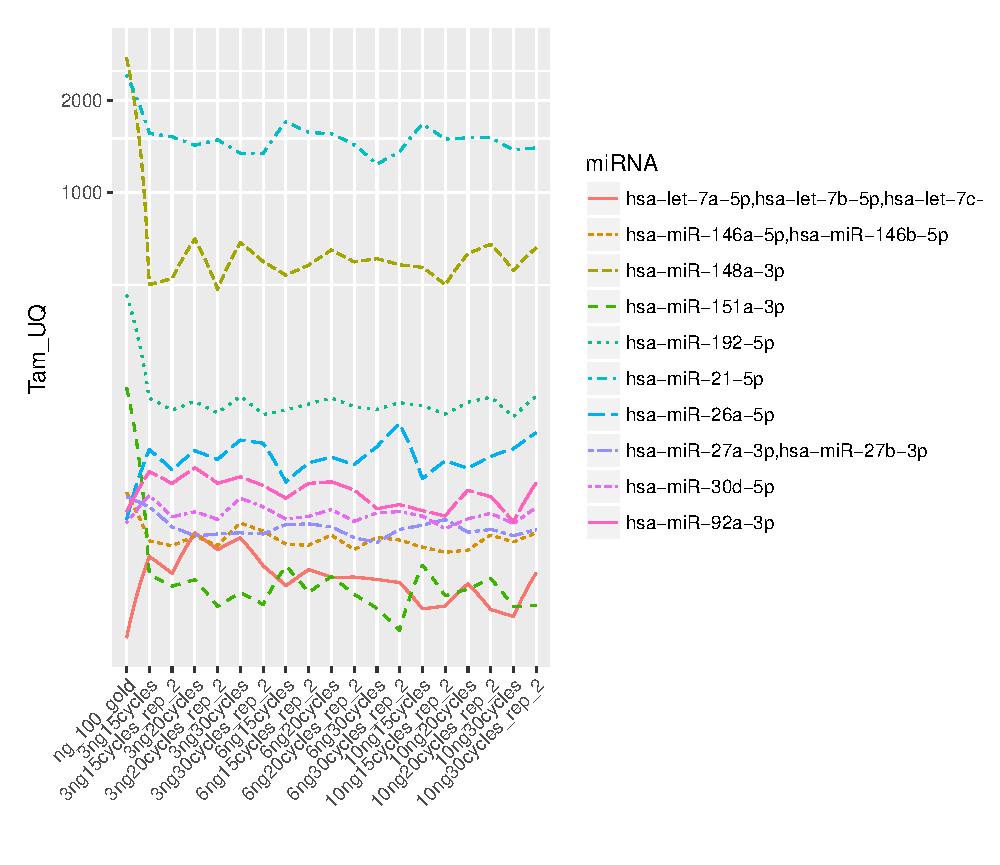
\includegraphics[scale=0.7]{fig-3-tamuq.eps}}
\caption{CPM Normalization}\label{fig:3}
\end{figure} 



\begin{figure}[!tpb]
\centerline{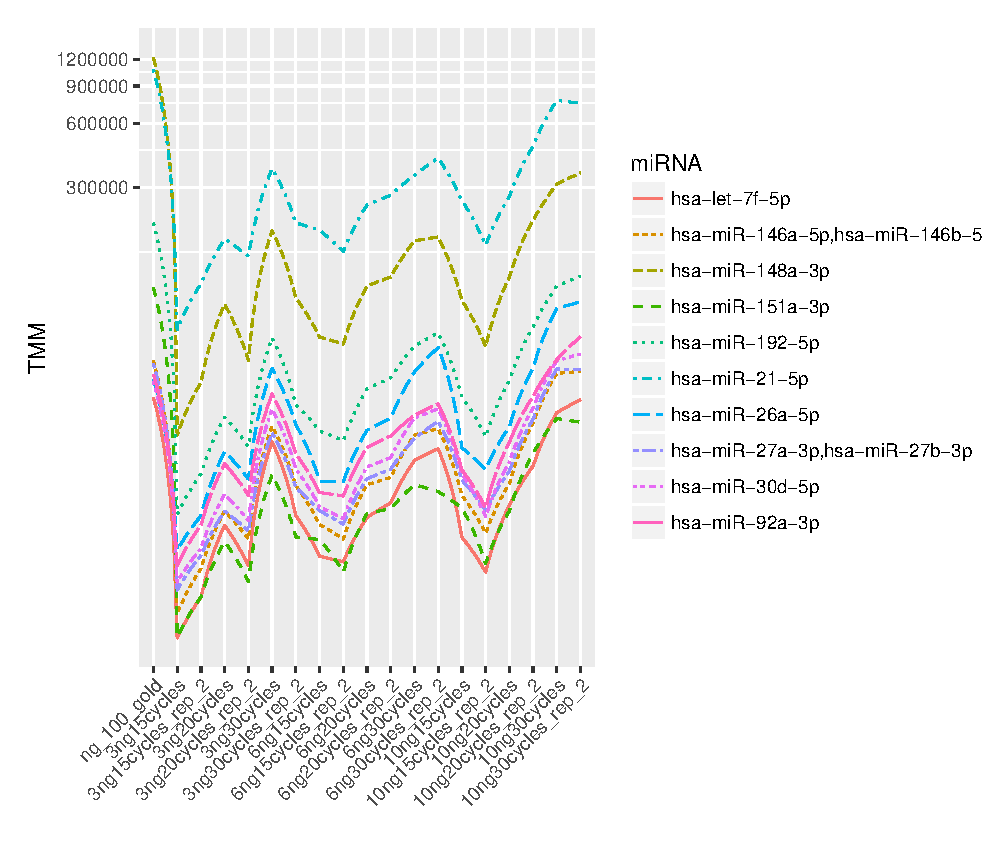
\includegraphics[scale=0.7]{fig-4-tmm.eps}}
\caption{TMM Normalization}\label{fig:4}
\end{figure} 




\begin{table}[ht]
\caption {Linear Model Coefficients} \label{tab:1}
\centering
\begin{tabular}{rlrrrrrr}
  \hline
 & miRNA & (Intercept) & sampleType10 & sampleType3 & sampleType6 & sampleCycleC20 & sampleCycleC30 \\ 
  \hline
1 & hsa-miR-21-5p & -0.47 & -0.41 & -0.59 & -0.42 & 0.05 & -0.03 \\ 
  2 & hsa-miR-148a-3p & -0.34 & -1.63 & -1.80 & -1.64 & 0.27 & 0.27 \\ 
  3 & hsa-miR-192-5p & -2.12 & -0.85 & -1.00 & -0.85 & 0.15 & 0.15 \\ 
  4 & hsa-miR-26a-5p & -3.81 & 0.37 & 0.26 & 0.39 & 0.18 & 0.35 \\ 
  5 & hsa-miR-92a-3p & -3.76 & 0.05 & 0.09 & 0.12 & 0.18 & 0.12 \\ 
  6 & hsa-miR-30d-5p & -3.84 & 0.02 & -0.06 & 0.04 & 0.12 & 0.18 \\ 
  7 & hsa-miR-27a-3p,hsa-miR-27b-3p & -3.64 & -0.19 & -0.34 & -0.20 & 0.03 & 0.05 \\ 
  8 & hsa-miR-146a-5p,hsa-miR-146b-5p & -3.61 & -0.43 & -0.53 & -0.41 & 0.14 & 0.23 \\ 
  9 & hsa-miR-151a-3p & -2.82 & -1.44 & -1.59 & -1.47 & 0.06 & -0.07 \\ 
  10 & hsa-let-7f-5p & -4.01 & -0.45 & -0.41 & -0.34 & 0.19 & 0.28 \\ 
  11 & hsa-let-7g-5p,hsa-let-7i-5p & -3.78 & -0.64 & -0.84 & -0.65 & 0.20 & 0.16 \\ 
  12 & hsa-let-7a-5p,hsa-let-7b-5p,hsa-let-7c-5p & -4.70 & 0.23 & 0.43 & 0.39 & 0.21 & 0.20 \\ 
   \hline
\end{tabular}
\end{table}

\begin{table}[ht]
\caption {miRNA features} \label{tab:2}
\centering
\begin{tabular}{lccrc}
  \hline
 miRNA &  Up or Down Regulated & Sequence & CG frac & Mfold Prediction  \\ 
  \hline
  hsa-let-7g-5p,hsa-let-7i-5p & UP & ugagguaguaguuuguacaguu & 0.36 & Linear \\
  hsa-miR-26a-5p   & UP & uucaaguaauccaggauaggcu & 0.41 & Linear \\
  hsa-miR-30d-5p   & UP & uguaaacauccccgacuggaag & 0.50  & Linear\\
  hsa-miR-146        & UP &  ugagaacugaauuccauggguu & 0.41  & Linear\\
  hsa-miR-151a-3p & DOWN & cuagacugaagcuccuugagg & 0.52  & Linear\\
  hsa-miR-192-5p & DOWN & cugaccuaugaauugacagcc & 0.48  & Linear\\
 \hline
\end{tabular}
\end{table}



\end{document}
%
%\begin{table}[!t]
%\processtable{This is table caption\label{Tab:01}} {\begin{tabular}{@{}llll@{}}\toprule head1 &
%head2 & head3 & head4\\\midrule
%row1 & row1 & row1 & row1\\
%row2 & row2 & row2 & row2\\
%row3 & row3 & row3 & row3\\
%row4 & row4 & row4 & row4\\\botrule
%\end{tabular}}{This is a footnote}
%\end{table}


%
%\begin{figure}[!tpb]%figure1
%\fboxsep=0pt\colorbox{gray}{\begin{minipage}[t]{235pt} \vbox to 100pt{\vfill\hbox to
%235pt{\hfill\fontsize{24pt}{24pt}\selectfont FPO\hfill}\vfill}
%\end{minipage}}
%%\centerline{\includegraphics{fig01.eps}}
%\caption{Caption, caption.}\label{fig:01}
%\end{figure}

%\begin{figure}[!tpb]%figure2
%%\centerline{\includegraphics{fig02.eps}}
%\caption{Caption, caption.}\label{fig:02}
%\end{figure}

%\enlargethispage{12pt}
%\enlargethispage{6pt}

%\bibliographystyle{natbib}
%\bibliographystyle{achemnat}
%\bibliographystyle{plainnat}
%\bibliographystyle{abbrv}
%\bibliographystyle{bioinformatics}
%
%\bibliographystyle{plain}
%
%\bibliography{Document}